\documentclass{beamer}
\usetheme[white]{Wisconsin}
\usepackage{longtable}
\usepackage{listings}
\usepackage{color}
%% The amssymb package provides various useful mathematical symbols
\usepackage{amssymb}
%% The amsthm package provides extended theorem environments
\usepackage{amsthm} \usepackage{amsmath} \usepackage{tmadd,tmath}
\usepackage[mathcal]{euscript} \usepackage{color}
\usepackage{textcomp}
\usepackage{algorithm,algorithmic}
\definecolor{listinggray}{gray}{0.9}
\definecolor{lbcolor}{rgb}{0.9,0.9,0.9}
\lstset{
  backgroundcolor=\color{lbcolor},
  tabsize=4,
  rulecolor=,
  language=c++,
  basicstyle=\scriptsize,
  upquote=true,
  aboveskip={1.5\baselineskip},
  columns=fixed,
  showstringspaces=false,
  extendedchars=true,
  breaklines=true,
  prebreak =
  \raisebox{0ex}[0ex][0ex]{\ensuremath{\hookleftarrow}},
  frame=single,
  showtabs=false,
  showspaces=false,
  showstringspaces=false,
  identifierstyle=\ttfamily,
  keywordstyle=\color[rgb]{0,0,1},
  commentstyle=\color[rgb]{0.133,0.545,0.133},
  stringstyle=\color[rgb]{0.627,0.126,0.941},
}

%% colors
\setbeamercolor{boxheadcolor}{fg=white,bg=UWRed}
\setbeamercolor{boxbodycolor}{fg=black,bg=white}


%%---------------------------------------------------------------------------%%
\author{\small Stuart R. Slattery and Paul P.H. Wilson, University of
  Wisconsin - Madison \bigskip \\ Roger P. Pawlowski, Sandia National
  Laboratories }

\date{\today} 
\title{The Data Transfer Kit: A Geometric Rendezvous-Based Tool for
  Multiphysics Data Transfer}
\begin{document}
\maketitle

%%---------------------------------------------------------------------------%%
\begin{frame}{Motivation}

  \begin{itemize}
  \item Desire tools to facilitate massively parallel multiphysics
    simulation within the Consortium for Advanced Simulation of LWRs
    (CASL)
    \bigskip
  \item Potentially complex data transfer required between
    non-matching grids in geometric and parallel space
    \bigskip
  \item No common framework (both software and mathematical) is
    leveraged by all codes
    \bigskip
  \item Algorithm-driven library needed
    \bigskip
  \item Decouple discretization and DOFs from the data transfer
    algorithms
  \end{itemize}

\end{frame}

%%---------------------------------------------------------------------------%%
\begin{frame}{What is DTK?}

  \begin{itemize}
  \item Collection of geometry-based data mapping algorithms for
    shared domain problems
    \bigskip
  \item Parallel topology maps allow for efficient movement of data in
    parallel (e.g. between meshes of a different parallel
    decomposition)
    \bigskip
  \item Ideally maps are generated at a desirable time complexity
    (logarithmic)
    \bigskip
  \item Input mesh and geometry data drive the map generation
    \bigskip
  \item Should be viewed as a service providing suite of concrete
    algorithm implementations for topology map generation
  \end{itemize}
 
\end{frame}

%%---------------------------------------------------------------------------%%
\begin{frame}{Software Overview}

  \begin{itemize}
  \item Preliminary development of mesh-based capabilities during
    summer 2012 CASL internship at ORNL
    \bigskip
  \item Additional development of geometry-based capabilities during
    fall 2012
    \bigskip
  \item Implemented in C++
    \bigskip
  \item Heavy use of the Trilinos scientific computing libraries
    \bigskip
  \item Open-source BSD 3-clause license
    \bigskip
  \item https://github.com/CNERG/DataTransferKit
  \end{itemize}
  
\end{frame}

%%---------------------------------------------------------------------------%%
\begin{frame}{Concepts and Geometric Rendezvous}

  \begin{itemize}
  \item Communicators
    \bigskip
  \item Shared Domain Problems
    \bigskip
  \item Parallel Topology Maps
    \bigskip
  \item The Rendezvous Algorithm
  \end{itemize}

\end{frame}

%%---------------------------------------------------------------------------%%
\begin{frame}{Communicators}

  \begin{columns}
    
    \begin{column}{0.5\textwidth}
      \begin{itemize}
      \item DTK handles source and target communicators of arbitrary
        relation 
        \bigskip
      \item Any amount of overlap or lack thereof supported
        \bigskip
      \item A global communicator required (doesn't have to be
        MPI\_COMM\_WORLD) 
      \end{itemize}
    \end{column}

    \begin{column}{0.5\textwidth}
      \begin{figure}[htpb!]
        \centering 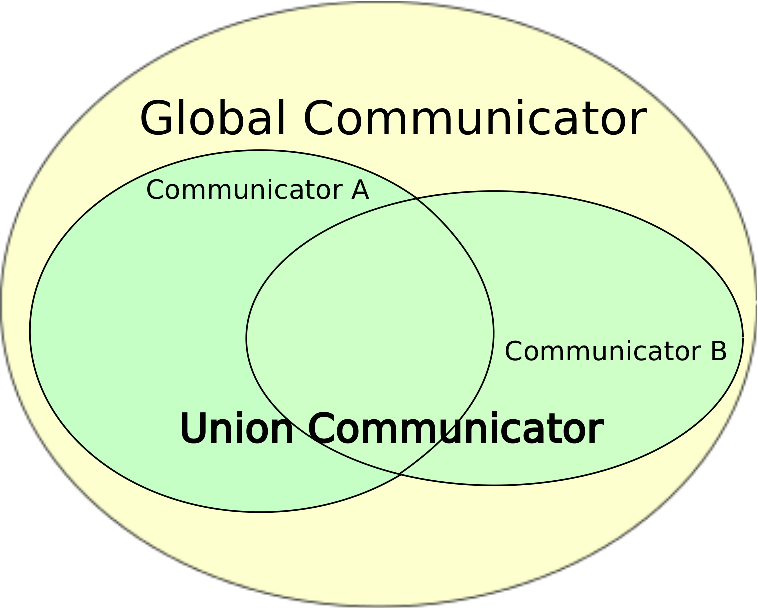
\includegraphics[width=1.7in]{union_comm.pdf}
      \end{figure}

      \begin{figure}[htpb!]
        \centering 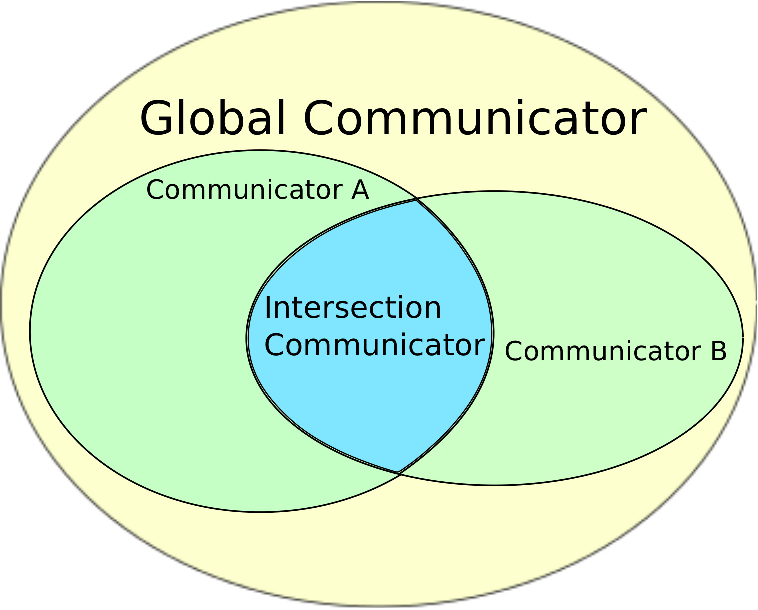
\includegraphics[width=1.7in]{intersection_comm.pdf}
      \end{figure}
    \end{column}

  \end{columns}

\end{frame}

%%---------------------------------------------------------------------------%%
\begin{frame}{Shared Domain Problems}

  \begin{columns}
    
    \begin{column}{0.5\textwidth}
      \begin{figure}[htpb!]
        \centering 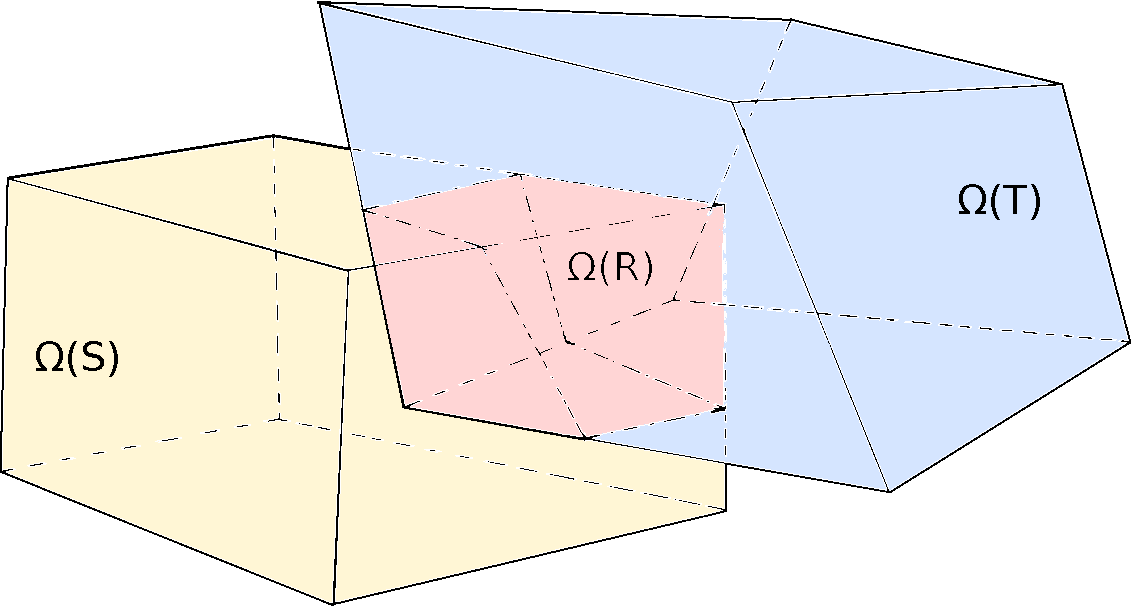
\includegraphics[width=2.5in]{overlapping_domain.pdf}
        \caption{\bf \sl Shared domain example.} {\sl $\Omega(S)$ (yellow)
          is the source geometry, $\Omega(T)$ (blue) is the target geometry,
          and $\Omega(R)$ (red) is the shared domain.}
        \label{fig:shared_domain}
      \end{figure}
    \end{column}

    \begin{column}{0.5\textwidth}
      \begin{itemize}
      \item Defined over a communicator that encapsulates the union of
        the source and target communicators
        \bigskip
      \item Source and target must be of same geometric dimension
        \bigskip
      \item The rendezvous algorithm leveraged to provide parallel
        topology maps for shared domains
      \end{itemize}
    \end{column}

  \end{columns}

\end{frame}

%%---------------------------------------------------------------------------%%
\begin{frame}{Parallel Topology Maps}
  
  An operator, $\ve{M}$, that defines the translation of a field,
  $\ve{F}(s)$, from a source spatial domain, $\Omega_S$, to a field,
  $\ve{G}(t$), in the target spatial domain $\Omega_T$, such that
  \[
  \ve{G}(t)\leftarrow \ve{M}(\ve{F}(s))
  \] 
  and 
  \[
  \ve{M}: \mathbb{R}^D \rightarrow \mathbb{R}^D, \forall r \in
  \Omega_R
  \]
  where $\Omega_R$ is the geometric rendezvous of the source and
  target
  \bigskip

  \begin{beamerboxesrounded}[upper=boxheadcolor,lower=boxbodycolor,shadow=true]
    {Notes}
    \begin{itemize}
    \item $\ve{M}$ is in general expensive to generate but cheap to
      apply
      \bigskip
    \item For static $\Omega_S$ and $\Omega_T$, building $\ve{M}$ is a
      one-time, upfront cost
    \end{itemize}
  \end{beamerboxesrounded}

\end{frame}

%%---------------------------------------------------------------------------%%
\begin{frame}{The Rendezvous Algorithm}

  \begin{itemize}
    \item Initially developed by the SIERRA team in the mid-2000's for
      parallel mesh-based data transfer \footnote{S. Plimpton,
        B. Hendrickson, and J. Stewart, “A parallel rendezvous
        algorithm for interpolation between multiple grids,” Journal
        of Parallel and Distributed Computing, vol. 64, pp. 266–276,
        2004}
      \medskip
    \item Creates a parallel topology map that can be used repeatedly
      for data transfer
    \item Map application uses asynchronous parallel strategy with
      minimal messages
    \item Effectively $N*log(N)$ time complexity for parallel topology
      map generation
      \medskip
    \item Relies on the generation of a secondary decomposition of the
      source and target meshes with a geometric-based partitioning
      (RCB)
  \end{itemize}

\end{frame}

%%---------------------------------------------------------------------------%%
\begin{frame}{The Rendezvous Decomposition}

  \begin{columns}

    \begin{column}{0.33\textwidth}
      \begin{figure}[htpb!]
        \centering 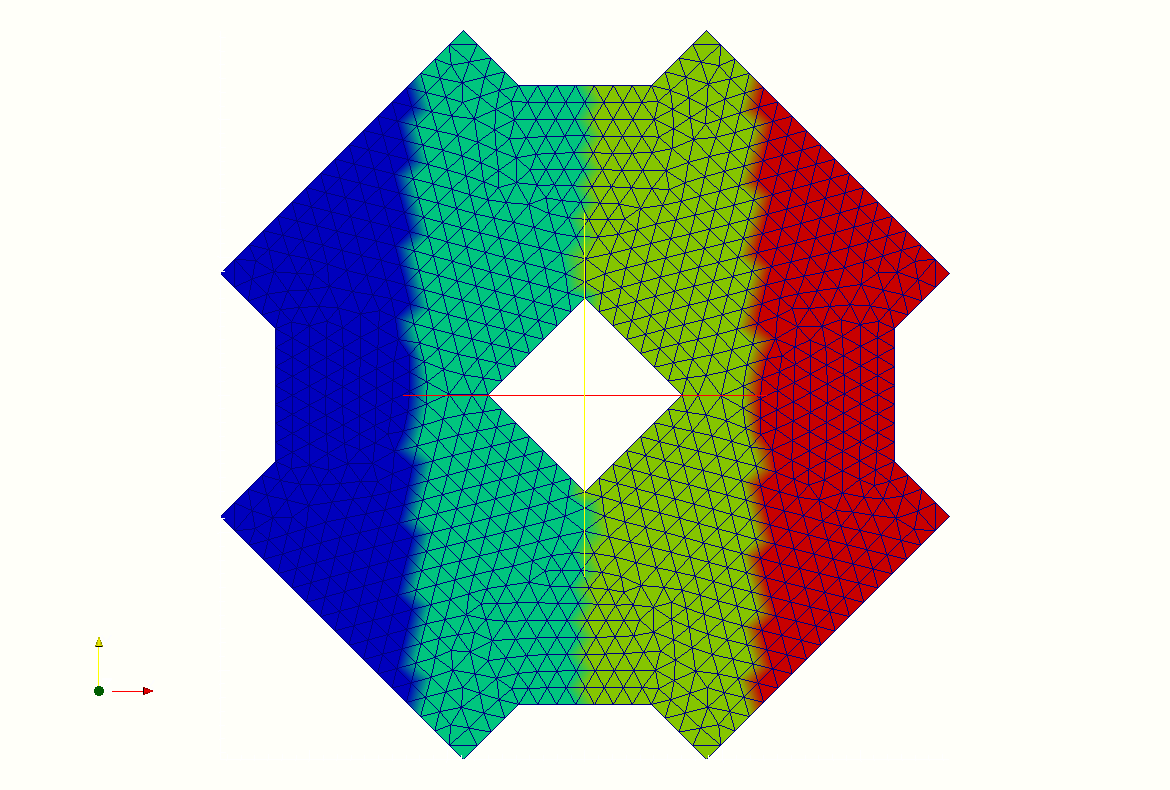
\includegraphics[width=2in]{tri_part.png}
        \caption{\small \sl Source mesh for 2D shared domain
          example.}
        \label{fig:source_mesh}
      \end{figure}
    \end{column}

    \begin{column}{0.33\textwidth}
      \begin{figure}[htpb!]
        \centering 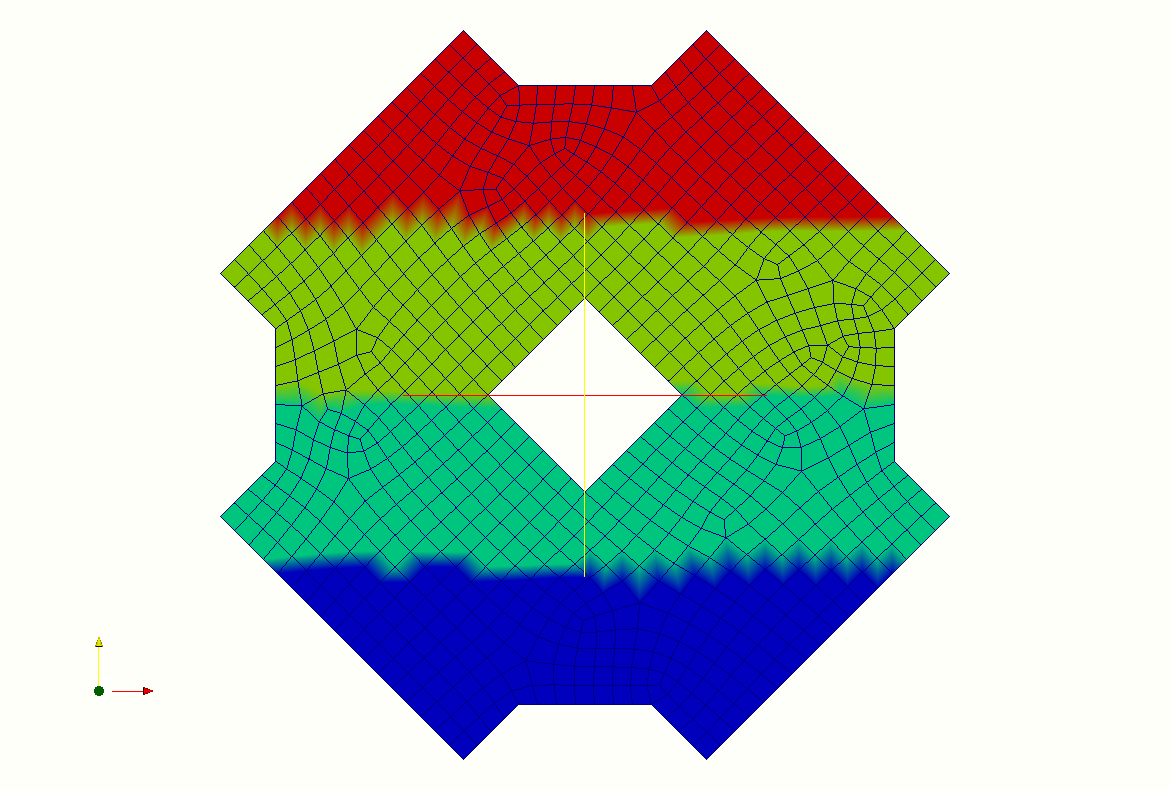
\includegraphics[width=2in]{quad_part.png}
        \caption{\small \sl Target mesh for 2D shared domain
          example.}
        \label{fig:target_mesh}
      \end{figure}
    \end{column}

    \begin{column}{0.33\textwidth}
      \begin{figure}[htpb!]
        \centering 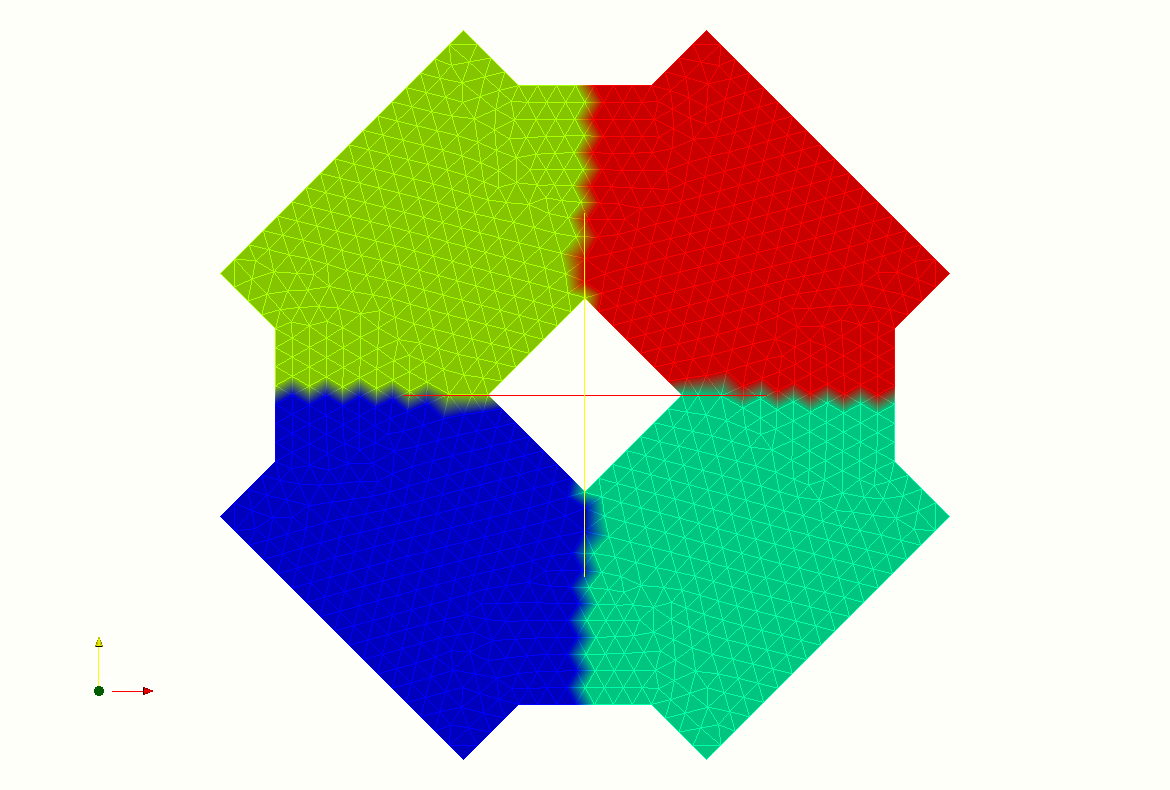
\includegraphics[width=2in]{tri_rend.png}
        \caption{\small \sl Rendezvous decomposition for 2D shared domain
          example.}
        \label{fig:rendezvous_part}
      \end{figure}
    \end{column}

  \end{columns}

\end{frame}

%%---------------------------------------------------------------------------%%
\begin{frame}{Searching the Rendezvous Decomposition}
  
  \begin{itemize}
  \item Hierarchical parallel search tree
    \bigskip
  \item Rendezvous decomposition provides parallel search
    \bigskip
  \item kD-tree provides on-process proximity search
    \bigskip
  \item Newton iterations provide final point location
    \bigskip
  \item Results in reasonable scalability
  \end{itemize}

\end{frame}

%%---------------------------------------------------------------------------%%
\begin{frame}{Field Evaluations for Map Application}

  \begin{itemize}
  \item Need to drive $\ve{G}(t)\leftarrow \ve{M}(\ve{F}(s))$
    \medskip
  \item Actual discretization of the field is not explicitly
    formulated
    \medskip
  \item Access to discretization of fields is generated through user
    code function evaluations at points in physical space:
    \medskip
  \end{itemize}

  \[
  \hat{f} \leftarrow \ve{F}(\hat{r}), \forall \hat{r} \in \Omega
  \]

  \begin{itemize}
  \item In the context of $\Omega$ discretized by a mesh, these
    evaluations can instead be written in terms of a single mesh
    element, $\omega \in \Omega$:
  \end{itemize}

  \[
  \hat{f} \leftarrow \ve{F}(\hat{r}), \forall \hat{r} \in \omega
  \]

\end{frame}

%%---------------------------------------------------------------------------%%
\begin{frame}{Neutronics/Thermal Hydraulics Verification}

  \begin{columns}
    
    \begin{column}{0.5\textwidth}
      \begin{figure}
      \centering
      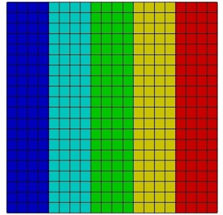
\includegraphics[width=1.25in]{neutronics_parallel_decomp.png}
      \end{figure}

      \begin{figure}
      \centering
      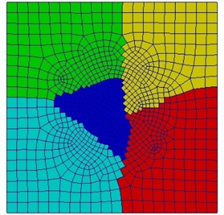
\includegraphics[width=1.25in]{cfd_parallel_decomp.png}
      \end{figure}
    \end{column}

    \begin{column}{0.5\textwidth}
      \begin{itemize}
      \item Mesh-to-Mesh transfer
        \medskip
      \item Used to move $\ve{F}(\hat{r})$ between meshes of arbitrary
        distribution
        \medskip
      \item Requires user code for evaluations in mesh elements
        \medskip
      \item 10-core ($2 \times 5$) calculation
      \end{itemize}

      \begin{figure}
      \centering
      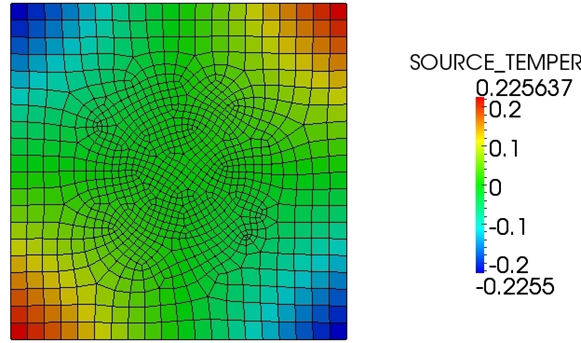
\includegraphics[width=1.75in]{cfd_transferred_field.png}
      \end{figure}
    \end{column}

  \end{columns}

\end{frame}

%%---------------------------------------------------------------------------%%
\begin{frame}{Field Integrations for Map Application}

  \begin{itemize}
  \item Consider a measure-weighted integral:
  \end{itemize}

  \[
  f_{\Omega} = \frac{\int_{\Omega} \ve{F}(r) dr}{\int_{\Omega} dr}
  \]

  \begin{itemize}
  \item In the context of $\Omega$ discretized by a mesh, these
    evaluations can instead be written in terms of a single mesh
    element, $\omega \in \Omega$:
  \end{itemize}

  \[
  f_{\omega} = \int_{\omega} \ve{F}(r) dr
  \]

  \begin{itemize}
  \item The integral over $\Omega$ will be the measure-weighted
    summation of all element integrals:
  \end{itemize}

  \[
    f_{\Omega} = \frac{1}{m_{\Omega}} \sum_i f_{{\omega}_i},\ \forall
    \omega_i \in \Omega
  \]

  \begin{itemize}
  \item Element-wise spatial integrals generated through user code
  \end{itemize}
\end{frame}

%%---------------------------------------------------------------------------%%
\begin{frame}{Other Rendezvous-Based Maps: Integral Assembly}

  \begin{columns}
    
    \begin{column}{0.4\textwidth}
      \begin{itemize}
      \item Mesh-to-geometry transfer
        \medskip
      \item Used to assemble $f_{\Omega}$ with mesh and geometry of
        arbitrary distribution into measure-weighted integral
        \medskip
      \item The mesh is assumed conformal
        \medskip
      \item Requires user code for integrations in mesh elements
      \end{itemize}
    \end{column}

    \begin{column}{0.6\textwidth}
      \begin{figure}
      \centering
      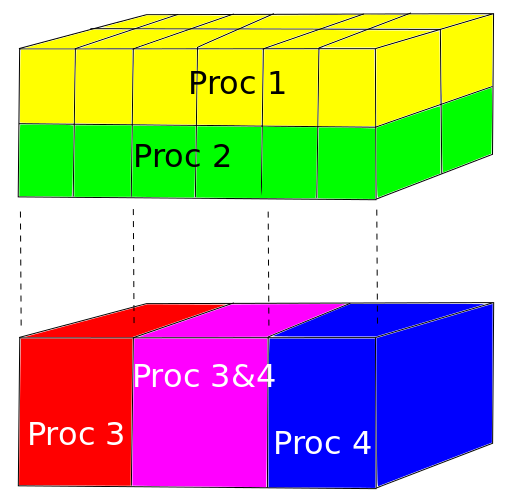
\includegraphics[width=2.5in]{integral_assembly.png}
      \end{figure}
    \end{column}

  \end{columns}

\end{frame}

%%---------------------------------------------------------------------------%%
\begin{frame}{DTK Implementation Scaling Results}

  \begin{columns}
    
    \begin{column}{0.5\textwidth}
      \begin{itemize}
      \item Mesh-to-mesh transfer
        \bigskip
      \item Worst case scenario study (all-to-all) with random points
        \bigskip
      \item Perfectly load balanced test
        \bigskip
      \item Qualitatively similar to the SIERRA results
        \bigskip
      \item Largest test problems so far over 1.0E9 elements and 1.0E5
        cores
      \end{itemize}
    \end{column}

    \begin{column}{0.5\textwidth}
      \begin{figure}
      \centering
      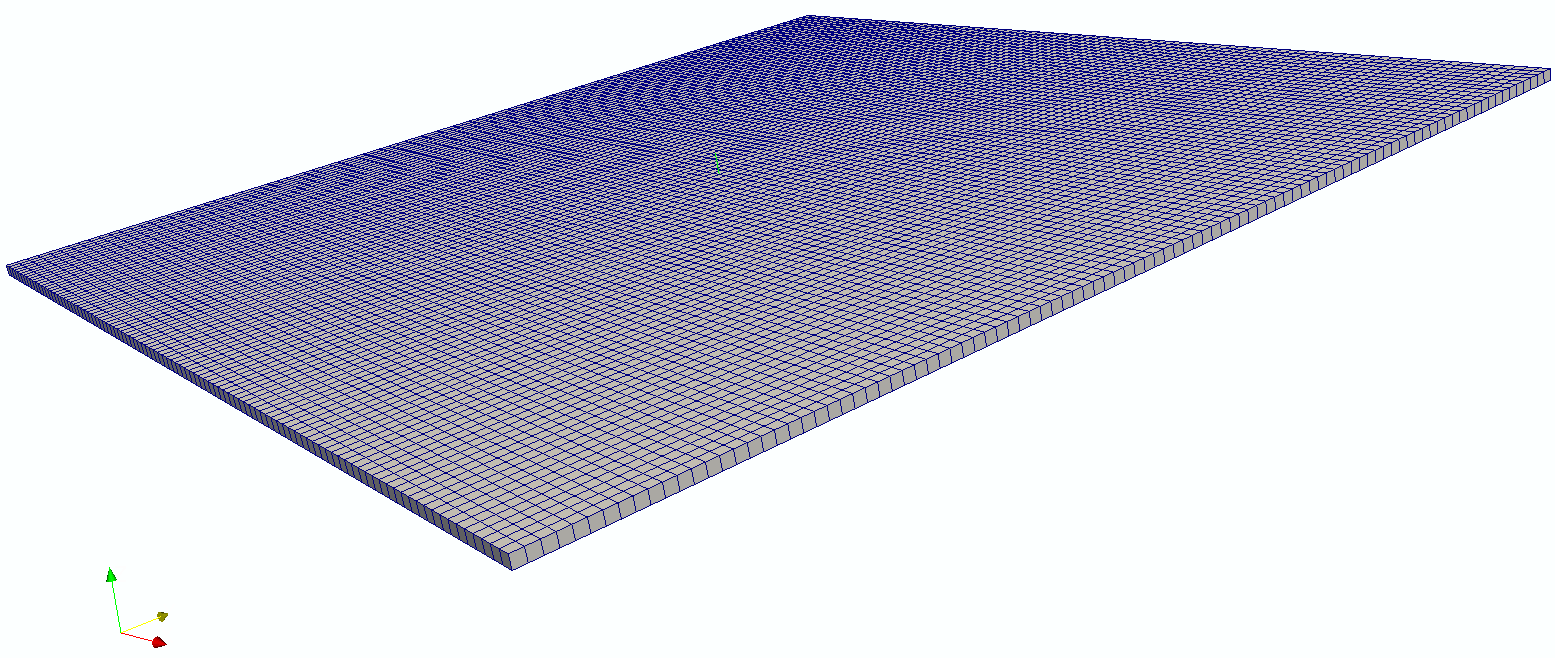
\includegraphics[width=2.4in]{mesh.png}
      \caption{\sl Local mesh partition for scaling studies. This
        partition has 1.0E4 tri-linear hexahedrons.}
      \end{figure}
    \end{column}

  \end{columns}

\end{frame}

%%---------------------------------------------------------------------------%%
\begin{frame}{Strong Scaling}

  \begin{figure}[htpb!]
    \centering
    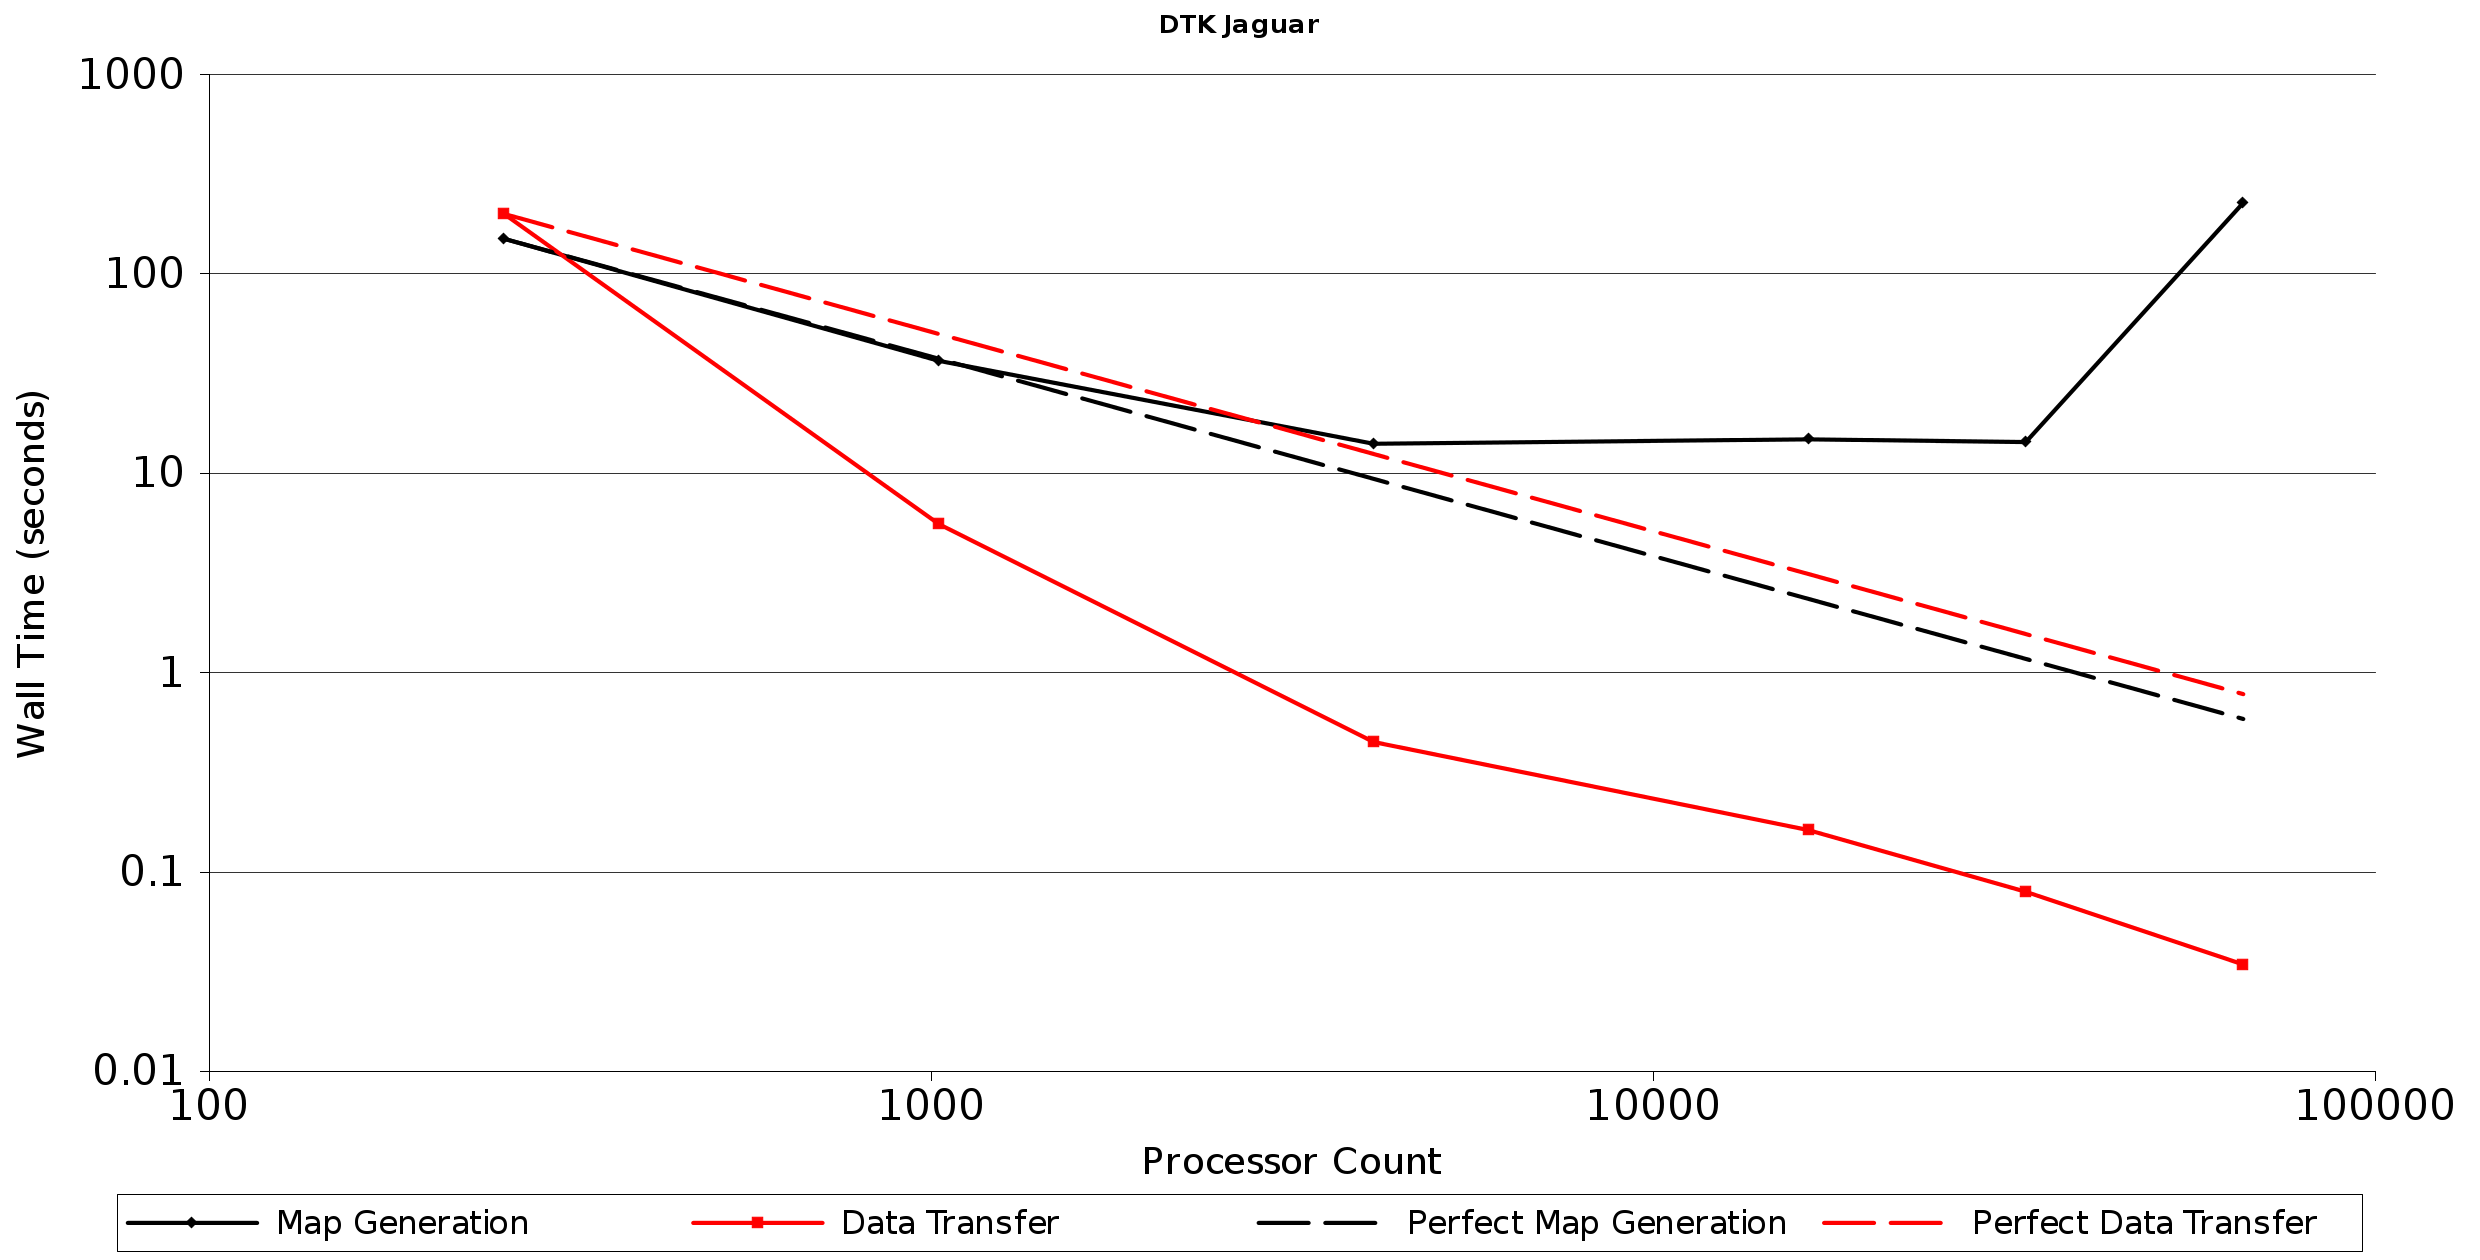
\includegraphics[width=4in]{StrongScaling.png}
    \caption{Strong scaling study results. The solid black curve reports
      the wall time to generate the mapping vs. number of processors
      while the solid red curve reports the wall time to transfer the
      data vs. number of processors. The dashed lines give
      perfect strong scaling the map generation (black) and the data
      transfer (red).}
    \label{fig:strong_scaling}
  \end{figure}

\end{frame}

%%---------------------------------------------------------------------------%%
\begin{frame}{Weak Scaling}

  \begin{figure}[ht!]
    \centering
    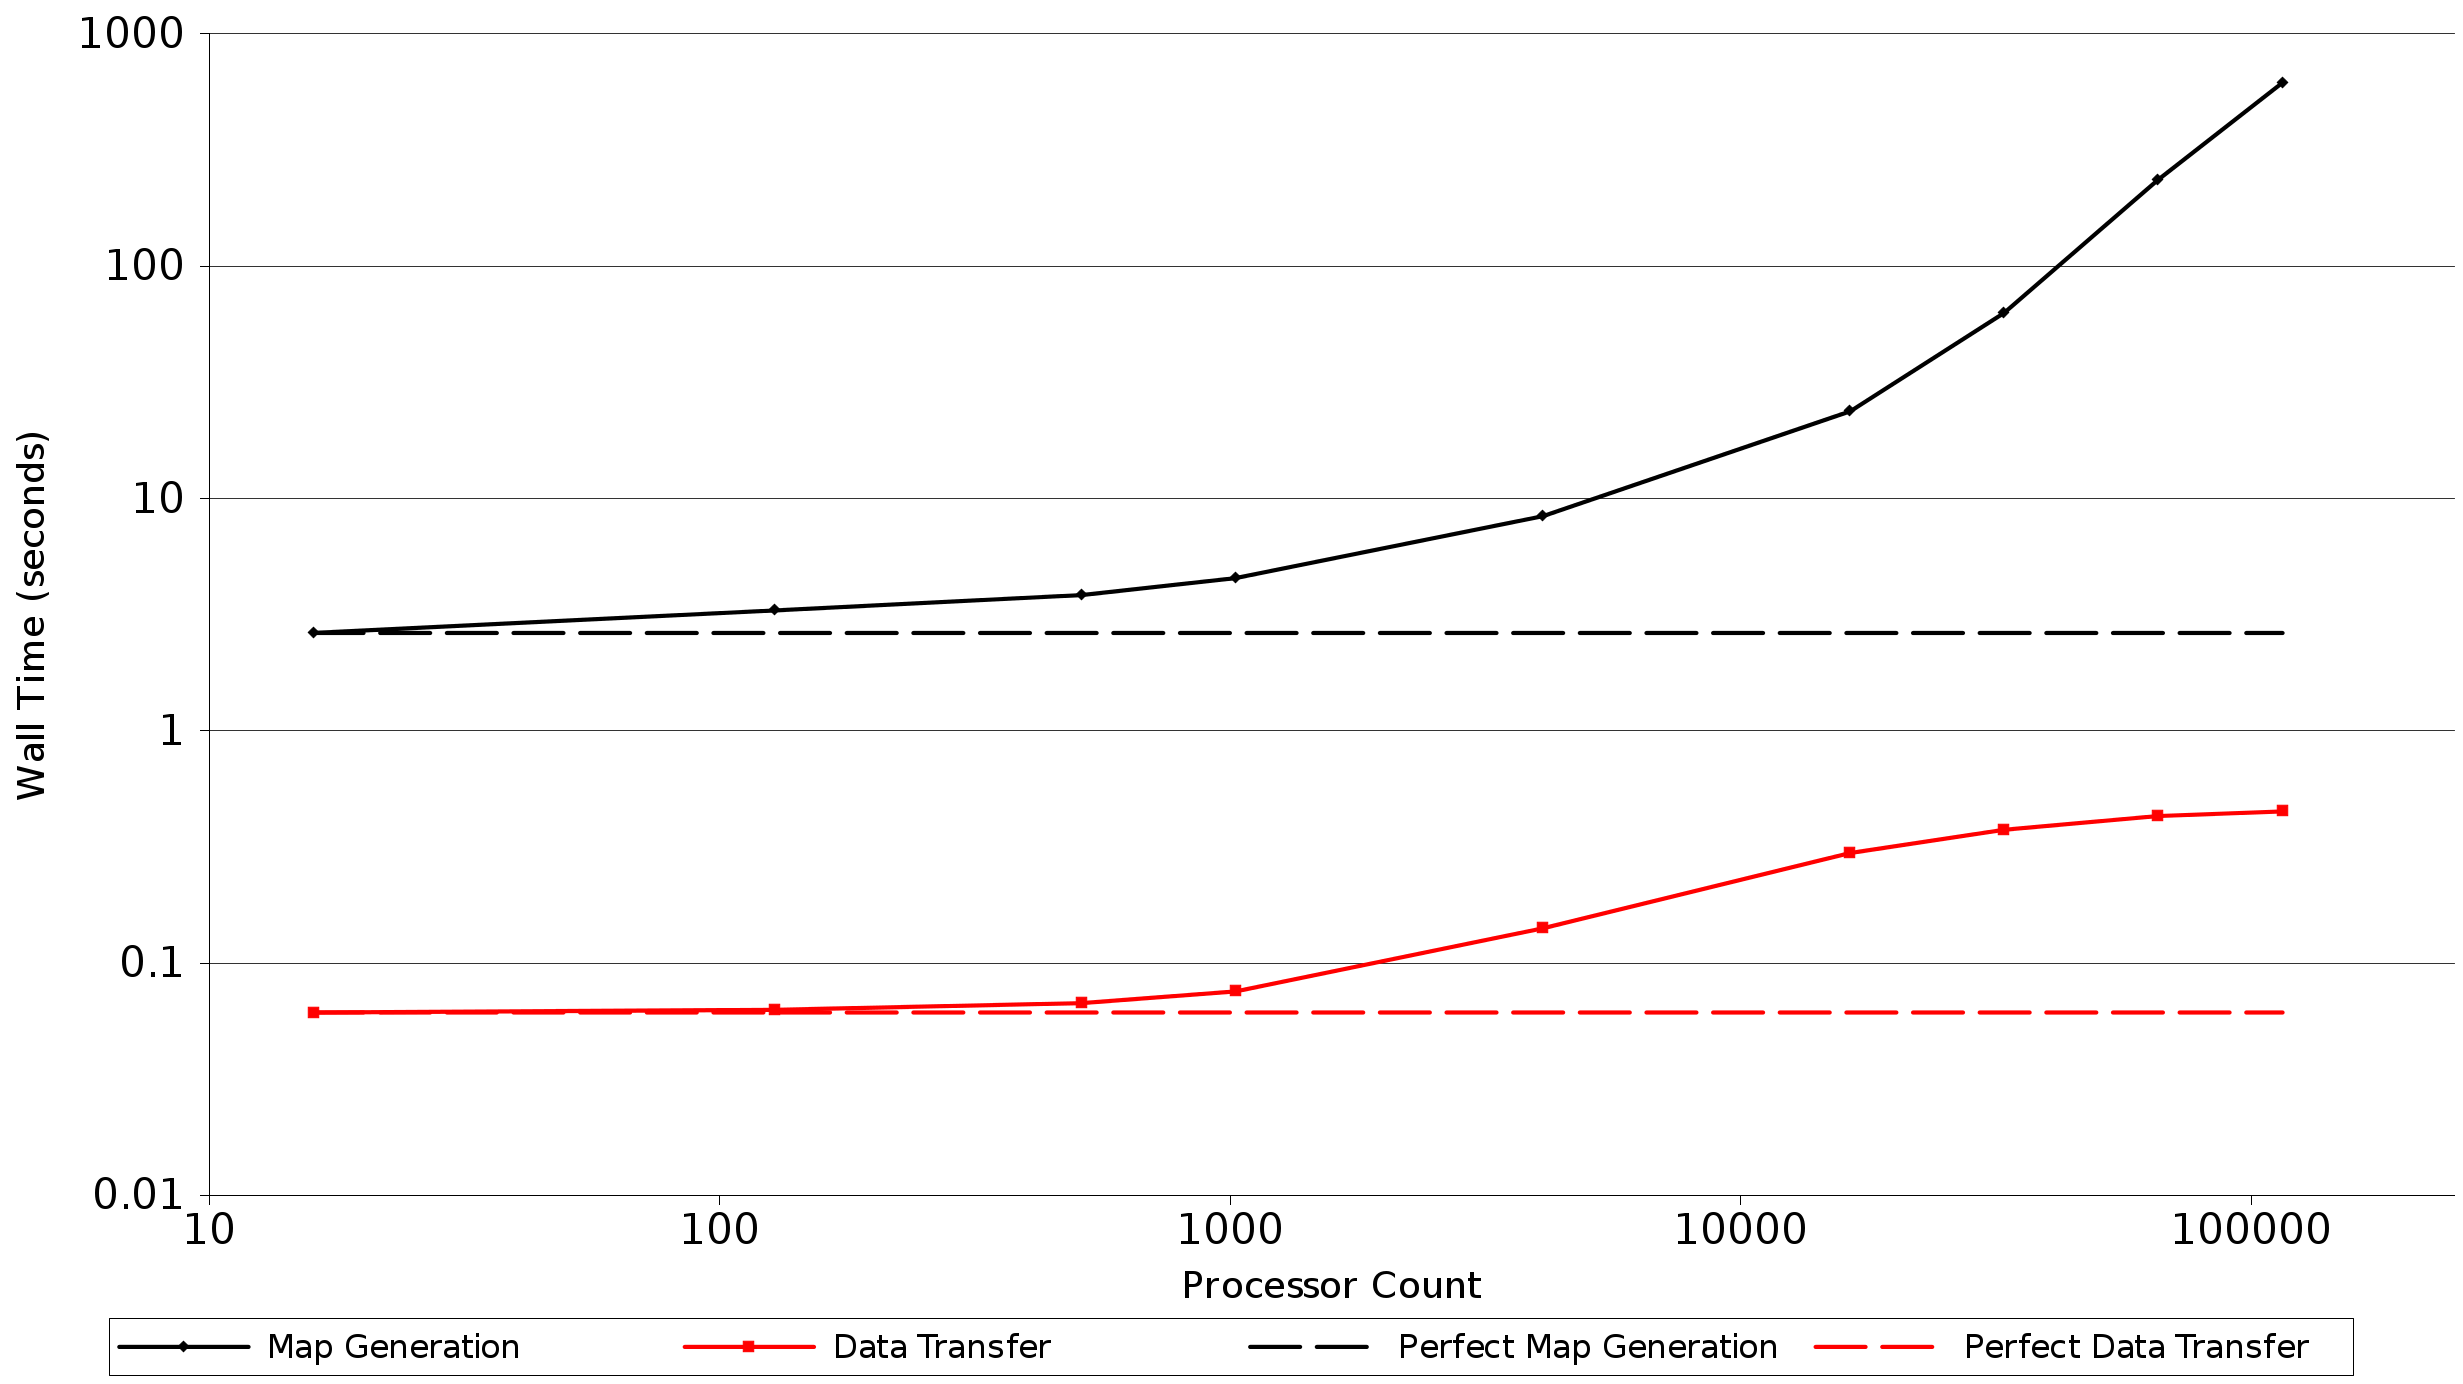
\includegraphics[width=4in]{WeakScaling.png}
    \caption{Weak scaling study results. The solid black curve reports
      the wall time to generate the mapping vs. number of processors
      while the solid red curve reports the wall time to transfer the
      data vs. number of processors. The dashed lines give
      perfect weak scaling the map generation (black) and the data
      transfer (red).}
    \label{fig:weak_scaling}
  \end{figure}

\end{frame}

%%---------------------------------------------------------------------------%%
\begin{frame}{Acknowledgements}

  \begin{itemize}
  \item This work was performed under funding provided by the
    Consortium for Advanced Simulation of LWRs (CASL)
    \bigskip
  \item The authors would like to thank the CASL Virtual Reactor
    Integration (VRI) development team for their assistance over the
    course of development of DTK
    \bigskip
  \item The authors would also like to thank the Oak Ridge Leadership
    Computing Facility (OLCF) for providing computational resources
    and support
  \end{itemize}

\end{frame}

%%---------------------------------------------------------------------------%%

\end{document}
